%  LaTeX support: latex@mdpi.com 
%  For support, please attach all files needed for compiling as well as the log file, and specify your operating system, LaTeX version, and LaTeX editor.

%=================================================================
\documentclass[remotesensing,article,submit,pdftex,moreauthors]{Definitions/mdpi} 

%--------------------
% Class Options:
%--------------------
%----------
% journal
%----------
% Choose between the following MDPI journals:
% acoustics, actuators, addictions, admsci, adolescents, aerobiology, aerospace, agriculture, agriengineering, agrochemicals, agronomy, ai, air, algorithms, allergies, alloys, analytica, analytics, anatomia, animals, antibiotics, antibodies, antioxidants, applbiosci, appliedchem, appliedmath, applmech, applmicrobiol, applnano, applsci, aquacj, architecture, arm, arthropoda, arts, asc, asi, astronomy, atmosphere, atoms, audiolres, automation, axioms, bacteria, batteries, bdcc, behavsci, beverages, biochem, bioengineering, biologics, biology, biomass, biomechanics, biomed, biomedicines, biomedinformatics, biomimetics, biomolecules, biophysica, biosensors, biotech, birds, bloods, blsf, brainsci, breath, buildings, businesses, cancers, carbon, cardiogenetics, catalysts, cells, ceramics, challenges, chemengineering, chemistry, chemosensors, chemproc, children, chips, cimb, civileng, cleantechnol, climate, clinpract, clockssleep, cmd, coasts, coatings, colloids, colorants, commodities, compounds, computation, computers, condensedmatter, conservation, constrmater, cosmetics, covid, crops, cryptography, crystals, csmf, ctn, curroncol, cyber, dairy, data, ddc, dentistry, dermato, dermatopathology, designs, devices, diabetology, diagnostics, dietetics, digital, disabilities, diseases, diversity, dna, drones, dynamics, earth, ebj, ecologies, econometrics, economies, education, ejihpe, electricity, electrochem, electronicmat, electronics, encyclopedia, endocrines, energies, eng, engproc, entomology, entropy, environments, environsciproc, epidemiologia, epigenomes, est, fermentation, fibers, fintech, fire, fishes, fluids, foods, forecasting, forensicsci, forests, foundations, fractalfract, fuels, future, futureinternet, futurepharmacol, futurephys, futuretransp, galaxies, games, gases, gastroent, gastrointestdisord, gels, genealogy, genes, geographies, geohazards, geomatics, geosciences, geotechnics, geriatrics, grasses, gucdd, hazardousmatters, healthcare, hearts, hemato, hematolrep, heritage, higheredu, highthroughput, histories, horticulturae, hospitals, humanities, humans, hydrobiology, hydrogen, hydrology, hygiene, idr, ijerph, ijfs, ijgi, ijms, ijns, ijpb, ijtm, ijtpp, ime, immuno, informatics, information, infrastructures, inorganics, insects, instruments, inventions, iot, j, jal, jcdd, jcm, jcp, jcs, jcto, jdb, jeta, jfb, jfmk, jimaging, jintelligence, jlpea, jmmp, jmp, jmse, jne, jnt, jof, joitmc, jor, journalmedia, jox, jpm, jrfm, jsan, jtaer, jvd, jzbg, kidneydial, kinasesphosphatases, knowledge, land, languages, laws, life, liquids, literature, livers, logics, logistics, lubricants, lymphatics, machines, macromol, magnetism, magnetochemistry, make, marinedrugs, materials, materproc, mathematics, mca, measurements, medicina, medicines, medsci, membranes, merits, metabolites, metals, meteorology, methane, metrology, micro, microarrays, microbiolres, micromachines, microorganisms, microplastics, minerals, mining, modelling, molbank, molecules, mps, msf, mti, muscles, nanoenergyadv, nanomanufacturing,\gdef\@continuouspages{yes}} nanomaterials, ncrna, ndt, network, neuroglia, neurolint, neurosci, nitrogen, notspecified, %%nri, nursrep, nutraceuticals, nutrients, obesities, oceans, ohbm, onco, %oncopathology, optics, oral, organics, organoids, osteology, oxygen, parasites, parasitologia, particles, pathogens, pathophysiology, pediatrrep, pharmaceuticals, pharmaceutics, pharmacoepidemiology,\gdef\@ISSN{2813-0618}\gdef\@continuous pharmacy, philosophies, photochem, photonics, phycology, physchem, physics, physiologia, plants, plasma, platforms, pollutants, polymers, polysaccharides, poultry, powders, preprints, proceedings, processes, prosthesis, proteomes, psf, psych, psychiatryint, psychoactives, publications, quantumrep, quaternary, qubs, radiation, reactions, receptors, recycling, regeneration, religions, remotesensing, reports, reprodmed, resources, rheumato, risks, robotics, ruminants, safety, sci, scipharm, sclerosis, seeds, sensors, separations, sexes, signals, sinusitis, skins, smartcities, sna, societies, socsci, software, soilsystems, solar, solids, spectroscj, sports, standards, stats, std, stresses, surfaces, surgeries, suschem, sustainability, symmetry, synbio, systems, targets, taxonomy, technologies, telecom, test, textiles, thalassrep, thermo, tomography, tourismhosp, toxics, toxins, transplantology, transportation, traumacare, traumas, tropicalmed, universe, urbansci, uro, vaccines, vehicles, venereology, vetsci, vibration, virtualworlds, viruses, vision, waste, water, wem, wevj, wind, women, world, youth, zoonoticdis 
% For posting an early version of this manuscript as a preprint, you may use "preprints" as the journal. Changing "submit" to "accept" before posting will remove line numbers.

%---------
% article
%---------
% The default type of manuscript is "article", but can be replaced by: 
% abstract, addendum, article, book, bookreview, briefreport, casereport, comment, commentary, communication, conferenceproceedings, correction, conferencereport, entry, expressionofconcern, extendedabstract, datadescriptor, editorial, essay, erratum, hypothesis, interestingimage, obituary, opinion, projectreport, reply, retraction, review, perspective, protocol, shortnote, studyprotocol, systematicreview, supfile, technicalnote, viewpoint, guidelines, registeredreport, tutorial
% supfile = supplementary materials

%----------
% submit
%----------
% The class option "submit" will be changed to "accept" by the Editorial Office when the paper is accepted. This will only make changes to the frontpage (e.g., the logo of the journal will get visible), the headings, and the copyright information. Also, line numbering will be removed. Journal info and pagination for accepted papers will also be assigned by the Editorial Office.

%------------------
% moreauthors
%------------------
% If there is only one author the class option oneauthor should be used. Otherwise use the class option moreauthors.

%---------
% pdftex
%---------
% The option pdftex is for use with pdfLaTeX. Remove "pdftex" for (1) compiling with LaTeX & dvi2pdf (if eps figures are used) or for (2) compiling with XeLaTeX.

%=================================================================
% MDPI internal commands - do not modify
\firstpage{1} 
\makeatletter 
\setcounter{page}{\@firstpage} 
\makeatother
\pubvolume{1}
\issuenum{1}
\articlenumber{0}
\pubyear{2023}
\copyrightyear{2023}
%\externaleditor{Academic Editor: Firstname Lastname}
\datereceived{ } 
\daterevised{ } % Comment out if no revised date
\dateaccepted{ } 
\datepublished{ } 
%\datecorrected{} % For corrected papers: "Corrected: XXX" date in the original paper.
%\dateretracted{} % For corrected papers: "Retracted: XXX" date in the original paper.
\hreflink{https://doi.org/} % If needed use \linebreak
%\doinum{}
%\pdfoutput=1 % Uncommented for upload to arXiv.org

%=================================================================
% Add packages and commands here. The following packages are loaded in our class file: fontenc, inputenc, calc, indentfirst, fancyhdr, graphicx, epstopdf, lastpage, ifthen, float, amsmath, amssymb, lineno, setspace, enumitem, mathpazo, booktabs, titlesec, etoolbox, tabto, xcolor, colortbl, soul, multirow, microtype, tikz, totcount, changepage, attrib, upgreek, array, tabularx, pbox, ragged2e, tocloft, marginnote, marginfix, enotez, amsthm, natbib, hyperref, cleveref, scrextend, url, geometry, newfloat, caption, draftwatermark, seqsplit
% cleveref: load \crefname definitions after \begin{document}
%=================================================================
% Please use the following mathematics environments: Theorem, Lemma, Corollary, Proposition, Characterization, Property, Problem, Example, ExamplesandDefinitions, Hypothesis, Remark, Definition, Notation, Assumption
%% For proofs, please use the proof environment (the amsthm package is loaded by the MDPI class).

%=================================================================
% Full title of the paper (Capitalized)
\Title{Rapid Processing and Georeferencing of Pushbroom Hyperspectral Imagery for Real Time Application by an Autonomous Aerial Vehicle}
%\Title{A Procedure for the Rapid Processing and Georeferencing of Hyperspectral Imagery for Real-Time use by an Autonomous Aerial Vehicle}
% MDPI internal command: Title for citation in the left column
\TitleCitation{Title}

% Author Orchid ID: enter ID or remove command
\newcommand{\orcidauthorA}{0000-0000-0000-000X} % Add \orcidA{} behind the author's name
%\newcommand{\orcidauthorB}{0000-0000-0000-000X} % Add \orcidB{} behind the author's name

% Authors, for the paper (add full first names)
\Author{John Waczak $^{1,\dagger,\ddagger}$\orcidA{}, David Lary $^{2,\ddagger}$ and Firstname Lastname $^{2,}$*}

%\longauthorlist{yes}

% MDPI internal command: Authors, for metadata in PDF
\AuthorNames{John Waczak, David Lary and Firstname Lastname}

% MDPI internal command: Authors, for citation in the left column
\AuthorCitation{Waczak, J.; Lary, D.; Lastname, F.}
% If this is a Chicago style journal: Lastname, Firstname, Firstname Lastname, and Firstname Lastname.

% Affiliations / Addresses (Add [1] after \address if there is only one affiliation.)
\address{%
$^{1}$ \quad Affiliation 1; e-mail@e-mail.com\\
$^{2}$ \quad Affiliation 2; e-mail@e-mail.com}

% Contact information of the corresponding author
\corres{Correspondence: e-mail@e-mail.com; Tel.: (optional; include country code; if there are multiple corresponding authors, add author initials) +xx-xxxx-xxx-xxxx (F.L.)}

% Current address and/or shared authorship
\firstnote{Current address: Affiliation 3.} 
\secondnote{These authors contributed equally to this work.}
% The commands \thirdnote{} till \eighthnote{} are available for further notes

%\simplesumm{} % Simple summary

%\conference{} % An extended version of a conference paper

% Abstract (Do not insert blank lines, i.e. \\) 
\abstract{Recent developments in hyperspectral imaging technology have led to dramatic reductions in both size and weight of imaging platforms. Due to these improvements, it is now possible to incorporate the technology as the payload of highly mobile autonomous aerial vehicles such as drones. However, the massive volume of hyperperspectral datacubes poses significant computational challenges to their adoption in real-time applications. In this paper, we demonstrate a procedure for the rapid georeferencing of pushbroom imagery and demonstrate its application for real-time remote sensing... Results indicate that a typical image can be processed in ~10 seconds while it takes $x$ seconds to capture. }

% Keywords
\keyword{keyword 1; keyword 2; keyword 3 (List three to ten pertinent keywords specific to the article; yet reasonably common within the subject discipline.)} 

% The fields PACS, MSC, and JEL may be left empty or commented out if not applicable
%\PACS{J0101}
%\MSC{}
%\JEL{}

%%%%%%%%%%%%%%%%%%%%%%%%%%%%%%%%%%%%%%%%%%
% Only for the journal Diversity
%\LSID{\url{http://}}

%%%%%%%%%%%%%%%%%%%%%%%%%%%%%%%%%%%%%%%%%%
% Only for the journal Applied Sciences
%\featuredapplication{Authors are encouraged to provide a concise description of the specific application or a potential application of the work. This section is not mandatory.}
%%%%%%%%%%%%%%%%%%%%%%%%%%%%%%%%%%%%%%%%%%

%%%%%%%%%%%%%%%%%%%%%%%%%%%%%%%%%%%%%%%%%%
% Only for the journal Data
%\dataset{DOI number or link to the deposited data set if the data set is published separately. If the data set shall be published as a supplement to this paper, this field will be filled by the journal editors. In this case, please submit the data set as a supplement.}
%\datasetlicense{License under which the data set is made available (CC0, CC-BY, CC-BY-SA, CC-BY-NC, etc.)}

%%%%%%%%%%%%%%%%%%%%%%%%%%%%%%%%%%%%%%%%%%
% Only for the journal Toxins
%\keycontribution{The breakthroughs or highlights of the manuscript. Authors can write one or two sentences to describe the most important part of the paper.}

%%%%%%%%%%%%%%%%%%%%%%%%%%%%%%%%%%%%%%%%%%
% Only for the journal Encyclopedia
%\encyclopediadef{For entry manuscripts only: please provide a brief overview of the entry title instead of an abstract.}

%%%%%%%%%%%%%%%%%%%%%%%%%%%%%%%%%%%%%%%%%%
% Only for the journal Advances in Respiratory Medicine
%\addhighlights{yes}
%\renewcommand{\addhighlights}{%

%\noindent This is an obligatory section in “Advances in Respiratory Medicine”, whose goal is to increase the discoverability and readability of the article via search engines and other scholars. Highlights should not be a copy of the abstract, but a simple text allowing the reader to quickly and simplified find out what the article is about and what can be cited from it. Each of these parts should be devoted up to 2~bullet points.\vspace{3pt}\\
%\textbf{What are the main findings?}
% \begin{itemize}[labelsep=2.5mm,topsep=-3pt]
% \item First bullet.
% \item Second bullet.
% \end{itemize}\vspace{3pt}
%\textbf{What is the implication of the main finding?}
% \begin{itemize}[labelsep=2.5mm,topsep=-3pt]
% \item First bullet.
% \item Second bullet.
% \end{itemize}
%}

%%%%%%%%%%%%%%%%%%%%%%%%%%%%%%%%%%%%%%%%%%
\begin{document}

%%%%%%%%%%%%%%%%%%%%%%%%%%%%%%%%%%%%%%%%%%

\section{Introduction}


For decades, multi-spectral imagers have seen wide spread adoption in the remote sensing community as a means to take advantage of the wealth of information contained in the reflectance spectra of materials. In addition to the three color filters of traditional cameras, multi-spectral imagers, like those deployed on MODIS, Landsat, Sentinel 2, and a plethora of other satellite missions, capture many additional features by utilizing wavelength bands ranging from the near-UV, through the visible spectrum, and into the Infrared. With this additional spectral information, multi-spectral remote sensing platforms are able to aid in a variety of domains like vegetation monitoring, land use classification, water quality assessment, smart agriculture, environmental change detection, and disaster management \textbf{(add references)}. 

\begin{figure}[H]
    \centering
    \includegraphics[width=15cm]{./assets/passbands.eps}
    \caption{Relative spectral response for the wavelength passbands of the popular multi-spectral remote sensing sources Sentinel 2A, Sentinel 2B, Landsat 8, and MODIS. Data from the USGS}
    \label{fig:passbands}
\end{figure}


These uses are justified by the reflectance features of materials across the electromagnetic spectrum; water has vibrational modes in the IR, pigments have absorption peaks in the visible, etc...(discuss the particular features present in different regions of the reflectance spectrum). Many currently used spectral indices like the *normalized difference vegatation index* (NDVI) take advantage of these spectral regions by comparing ratios of pigment sensitive passbands to the constant signals infrared to infer the abundance of chlorophyll, and consequently, the health of plants, to identify forest canopy, etc..(**add citations and expand**)

However, despite the plethora of successful applications of multi-spectral imaging, more can be accomplished with the additional information provided by fully resolved spectra. For example, in the laboratory, spectrophotometry allows the direct determination of the concentrations of chemicals constituents in solution (**add more detail and references**) by deconvolution of a sample spetrum against libraries carefully collected of reference spectra: individual chemicals be uniquely identified by the characterstic location and shape of their absorption features. We should mention something about algal blooms-- harmful species display shifted reflectance peaks that can be used to identify toxic species. This information is effectively filtered away by the broad passbands of existing (find the spectra used in that book that show the different species of algae). To that end, *hyperspectral imagers* (HSI), which sample hundreds of wavelength binds at each pixel, have become the natural next step for remote sensing platforms with many planned to deployed in the coming years (**add references about soon-to-be-deployed HSI satellites**). 


At the terrestrial level, drones (commonly, quadcoptrs, octocopters, and other similar multi-rotor craft) equipped with cameras are able to utlize techniques of photogrametry together with continuously sampled imagery to produce high quality digital elevation maps, high quality mosaics, 3-dimensional reconstructions, etc... These capabilities provide significant aid for structural analysis, smart agriculture, etc... Today, kilogram-scale HSI can be comfortably mounted to the payload of film-scale drones such as the AltaX and advancements in spectral sensing such as (**reference Ethan Minot's recent paper**) suggest that sizes of HSI will continue to shrink further expanding their application in this domain. 

The increased spectral resolution of HSI systems poses unique challenges to their adoption for real time applications primarily stemming from the considerable size of generated data files. Current data collection workflows see researchers first perform the aerial survey (data collection) and then transfer data to ground based computers for post processing. This workflow is well established in the remote sensing community where, as an example, compressed raw imagery from Sentinel-2 are transferred to the ground and then subsequently post processed into their final L1C (top of atmosphere) and L2A (bottom of atmosphere) data products ((**add citation here**)). Drone based applications often operate in a similar manner: images or video are collected by a survey and then post-processed and analyzed with software such as Open Drone Map to produce the desired data products (tile mosaics, 3d reconstructions, etc.) (**add citation**). For an HSI platform to function in real time, three key computational tasks are critical: 
1. **FileIO**: captured imagery need to be quickly read by the on-board processing computer
2. **Post-processing**: Raw imagery need to be rapidly converted to the chosen data product (typically, Reflectance), and importantly, must be georeferenced so that each image pixel can be located on the ground.
3. **Ground Transfer**: Sufficient wireless communication must be avaiable to transmit the final 

The first can be readily accomplished by means of light weight, high volume solid state drives. To address the second, we need both sufficient compute and optimized processing software. Finally, ground transfer of final post-processed data products can be accomplished in a variety of ways. As we rarely need the full hyper-spectral datacube right away, once can generate the desired data products on board (NDVI for example) and transfer only the relevant information to a ground station 

We should now make the argument about the need for improved methods for processing of HSI due the their dramatically larger size, i.e. the standard workflow of collecting imagery and then post processing (re: Open Drone Map) is a fantastic and well tested solution but prevents the use in time-critical applications. We can also reference the continued improvements to single-board computers such as the raspberry pi 4b (8 Gb of Ram), Jetson family (GPU equipped), and intel nuc (powerful work horses with miniscule form factors). To make real-time possible we need two things: 
1. Conversion from raw data (digital counts) to physical units like Reflectance 
2. Georeferencing of captured imagery so features can be quickly geolocated

We can always re-process the imagery later for an in-depth reanalysis, but for time-critical applications, we need all of the processing to happen on board the drone. 


Add a paragraph about georeferencing in particular:
- Georectification = georeference + orthorectification
- outline other papers that have discussed georectification techniques:
    - ground control points  (not reasonable for dangerous or water-based environments)
    - IMU / GPS
    - different type of sensors: square, pushbroom, whiskbroom

Discuss configurations of imagers and the development of georeferencing strategies, e.g. starting with the Muller paper and going to today. Mention potential for the incorporation of digital elevation maps together enabled by GPUs and video game engines (**reference that one paper that suggests using Unity or something similar for the projective geometry optimized for Cuda on NVIDIA GPUs**).

In our previous work, we demonstrated a prototype autonomous robot team employing a drone based hyper-spectral imager which can learn the mapping from reflectance spectra to concentrations of variety of chemicals-of-concern by utilizing the information contained in the reflectance spectra captured with a HSI together with a  \cite{robot-team-1}. In this paper, we present a procedure based on the method of \cite{muller-georeferencing} for the rapid processing and georeferencing of imagery captured by a pushbroom HSI mounted on an autonomous. Associated code can be freely accessed and downloaded in (**add reference to our repository**)

(**This point can be saved for the supervised learning paper**) what we really want (usually) isn't the full spectra at each pixel 

IMU - inertial measurement unit



%%%%%%%%%%%%%%%%%%%%%%%%%%%%%%%%%%%%%%%%%%
\section{Materials and Methods}

Make sure to use \textit{nadir-oriented} in description of HSI on the drone. 

\subsection{Autonomous Aerial Vehicle}

subsection detailing the robot team, and specifically, the drone setup (HSI, NUC, Flir, etc...) 
- HSI takes images 
- IMU/GPS onboard position/orientation determination
- Intel NUC 1: manages HSI
- SSD
- Intel NUC 2: Processing 
- Ubiquity long-range wifi antenna (for streaming data products)

\begin{figure}[H]
    \centering
    \includegraphics[width=12cm]{./assets/annotated-drone.eps}
    \caption{Components of the Autonomous Drone HSI platform.}
    \label{fig:drone-components}
\end{figure}


\subsection{Real time processing of HSI imagery}

- overview of processing pipeline

\begin{figure}[H]
    \centering
    \includegraphics[width=10.5cm]{./figures/pipeline-figure.eps}
    \caption{Solar Irradiance spectrum captured by downwelling spectrometer.}
    \label{fig:annotated-hsi}
\end{figure}

- Collection of raw HSI by imager
- Reading stored binary (ENVI) radiance data into tensor
- Reading Flight Data 
- Interpolate flight data from IMU to match HSI times
- Reading stored downwelling irradiance spectrum 
- Interpolate irradiance spectrum to match HSI $\lambda$s 
- Conversion to Reflectance under the assumption of a Lambertian surface (perfectly diffuse)
- Georectify to obtain new coordinates
- resample to regular grid
- compute derived $\lambda$-metrics (NDVI, etc...) 
- serve result (save to HDF5 or serve via web map service over wifi) 


Georectification Procedure.
\begin{itemize}
    \item collect datacube 
    \item read HSI in ENVI format
    \item read Flight Data 
    \item interpolate flight data to HSI times 
    \item read Downwelling irradiance spectrum
    \item convert radiance to reflectance 
    \item georectify to obtain new coordinates 
    \item resample to regular grid
    \item save results to HDF5
\end{itemize}

Code and data availability via OSN and Github



\subsection{Georectification Procedure}


\begin{figure}[H]
    \centering
    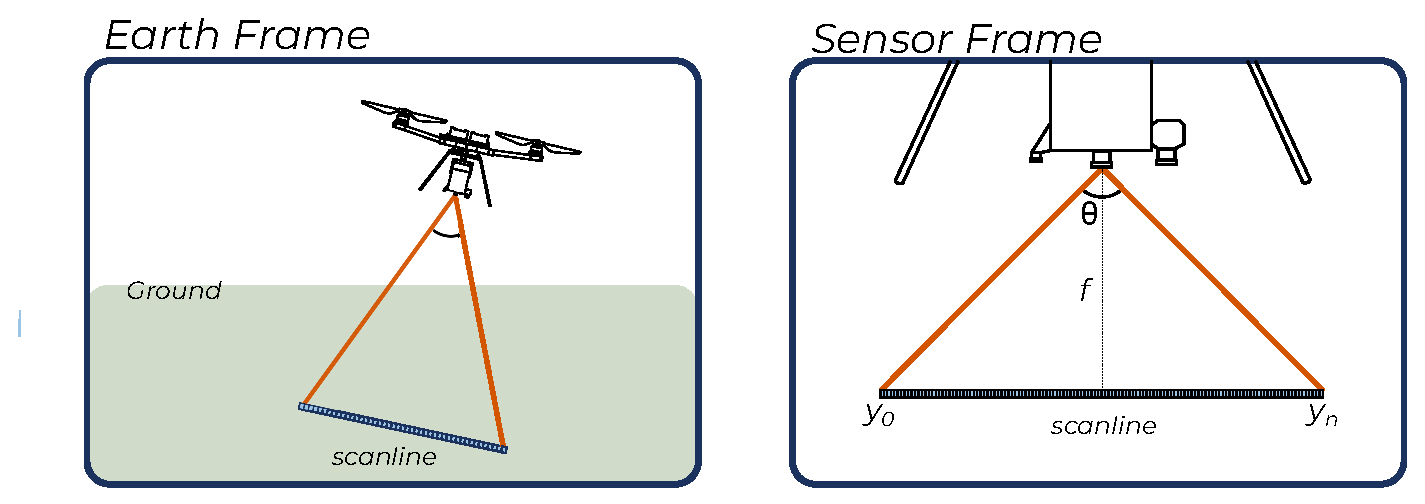
\includegraphics[width=10.5cm]{./assets/georectification.eps}
    \caption{Visual representation of scan-line geometry for the drone based hyperspectral imaging platform.}
    \label{fig:georectification}
\end{figure}





%%%%%%%%%%%%%%%%%%%%%%%%%%%%%%%%%%%%%%%%%%
\section{Results}

\begin{figure}[H]
    \begin{adjustwidth}{-\extralength}{0cm}
        \centering
        \includegraphics[width=15.5cm]{./figures/hsi-infographic.eps}
    \end{adjustwidth}
    \caption{Annotated view of a hyperspectral data cube showcasing sampled spectra for a variety of constituents.\label{fig:hsi-infographic}}
\end{figure}  


\begin{figure}[H]
    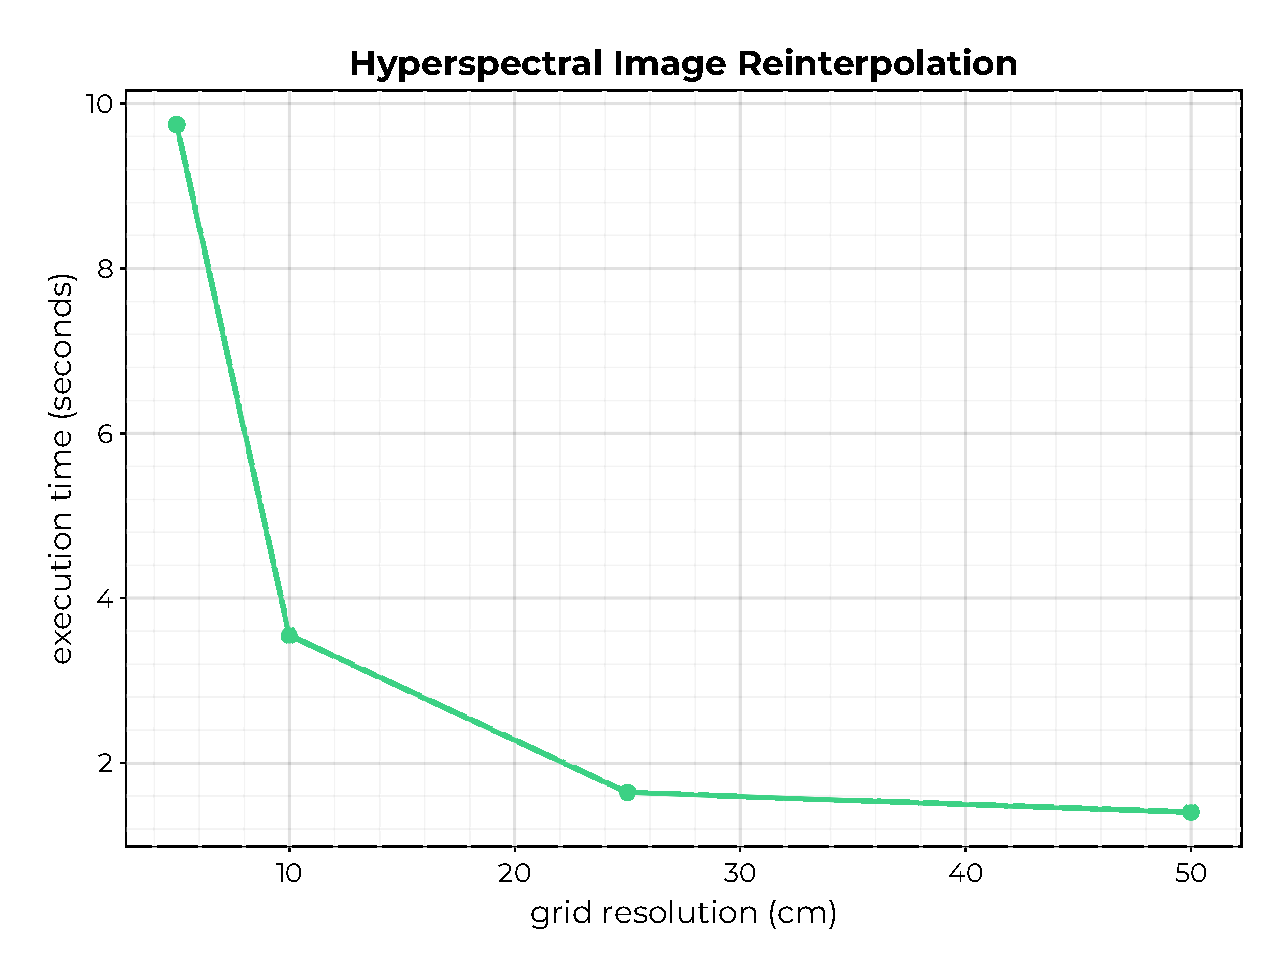
\includegraphics[width=10.5 cm]{./figures/regrid-timing.eps}
\caption{This is a figure. Schemes follow the same formatting. If there are multiple panels, they should be listed as: (\textbf{a}) Description of what is contained in the first panel. (\textbf{b}) Description of what is contained in the second panel. Figures should be placed in the main text near to the first time they are cited. A caption on a single line should be centered.\label{fig-regridding-timing}}
\end{figure}

\begin{figure}[H]
  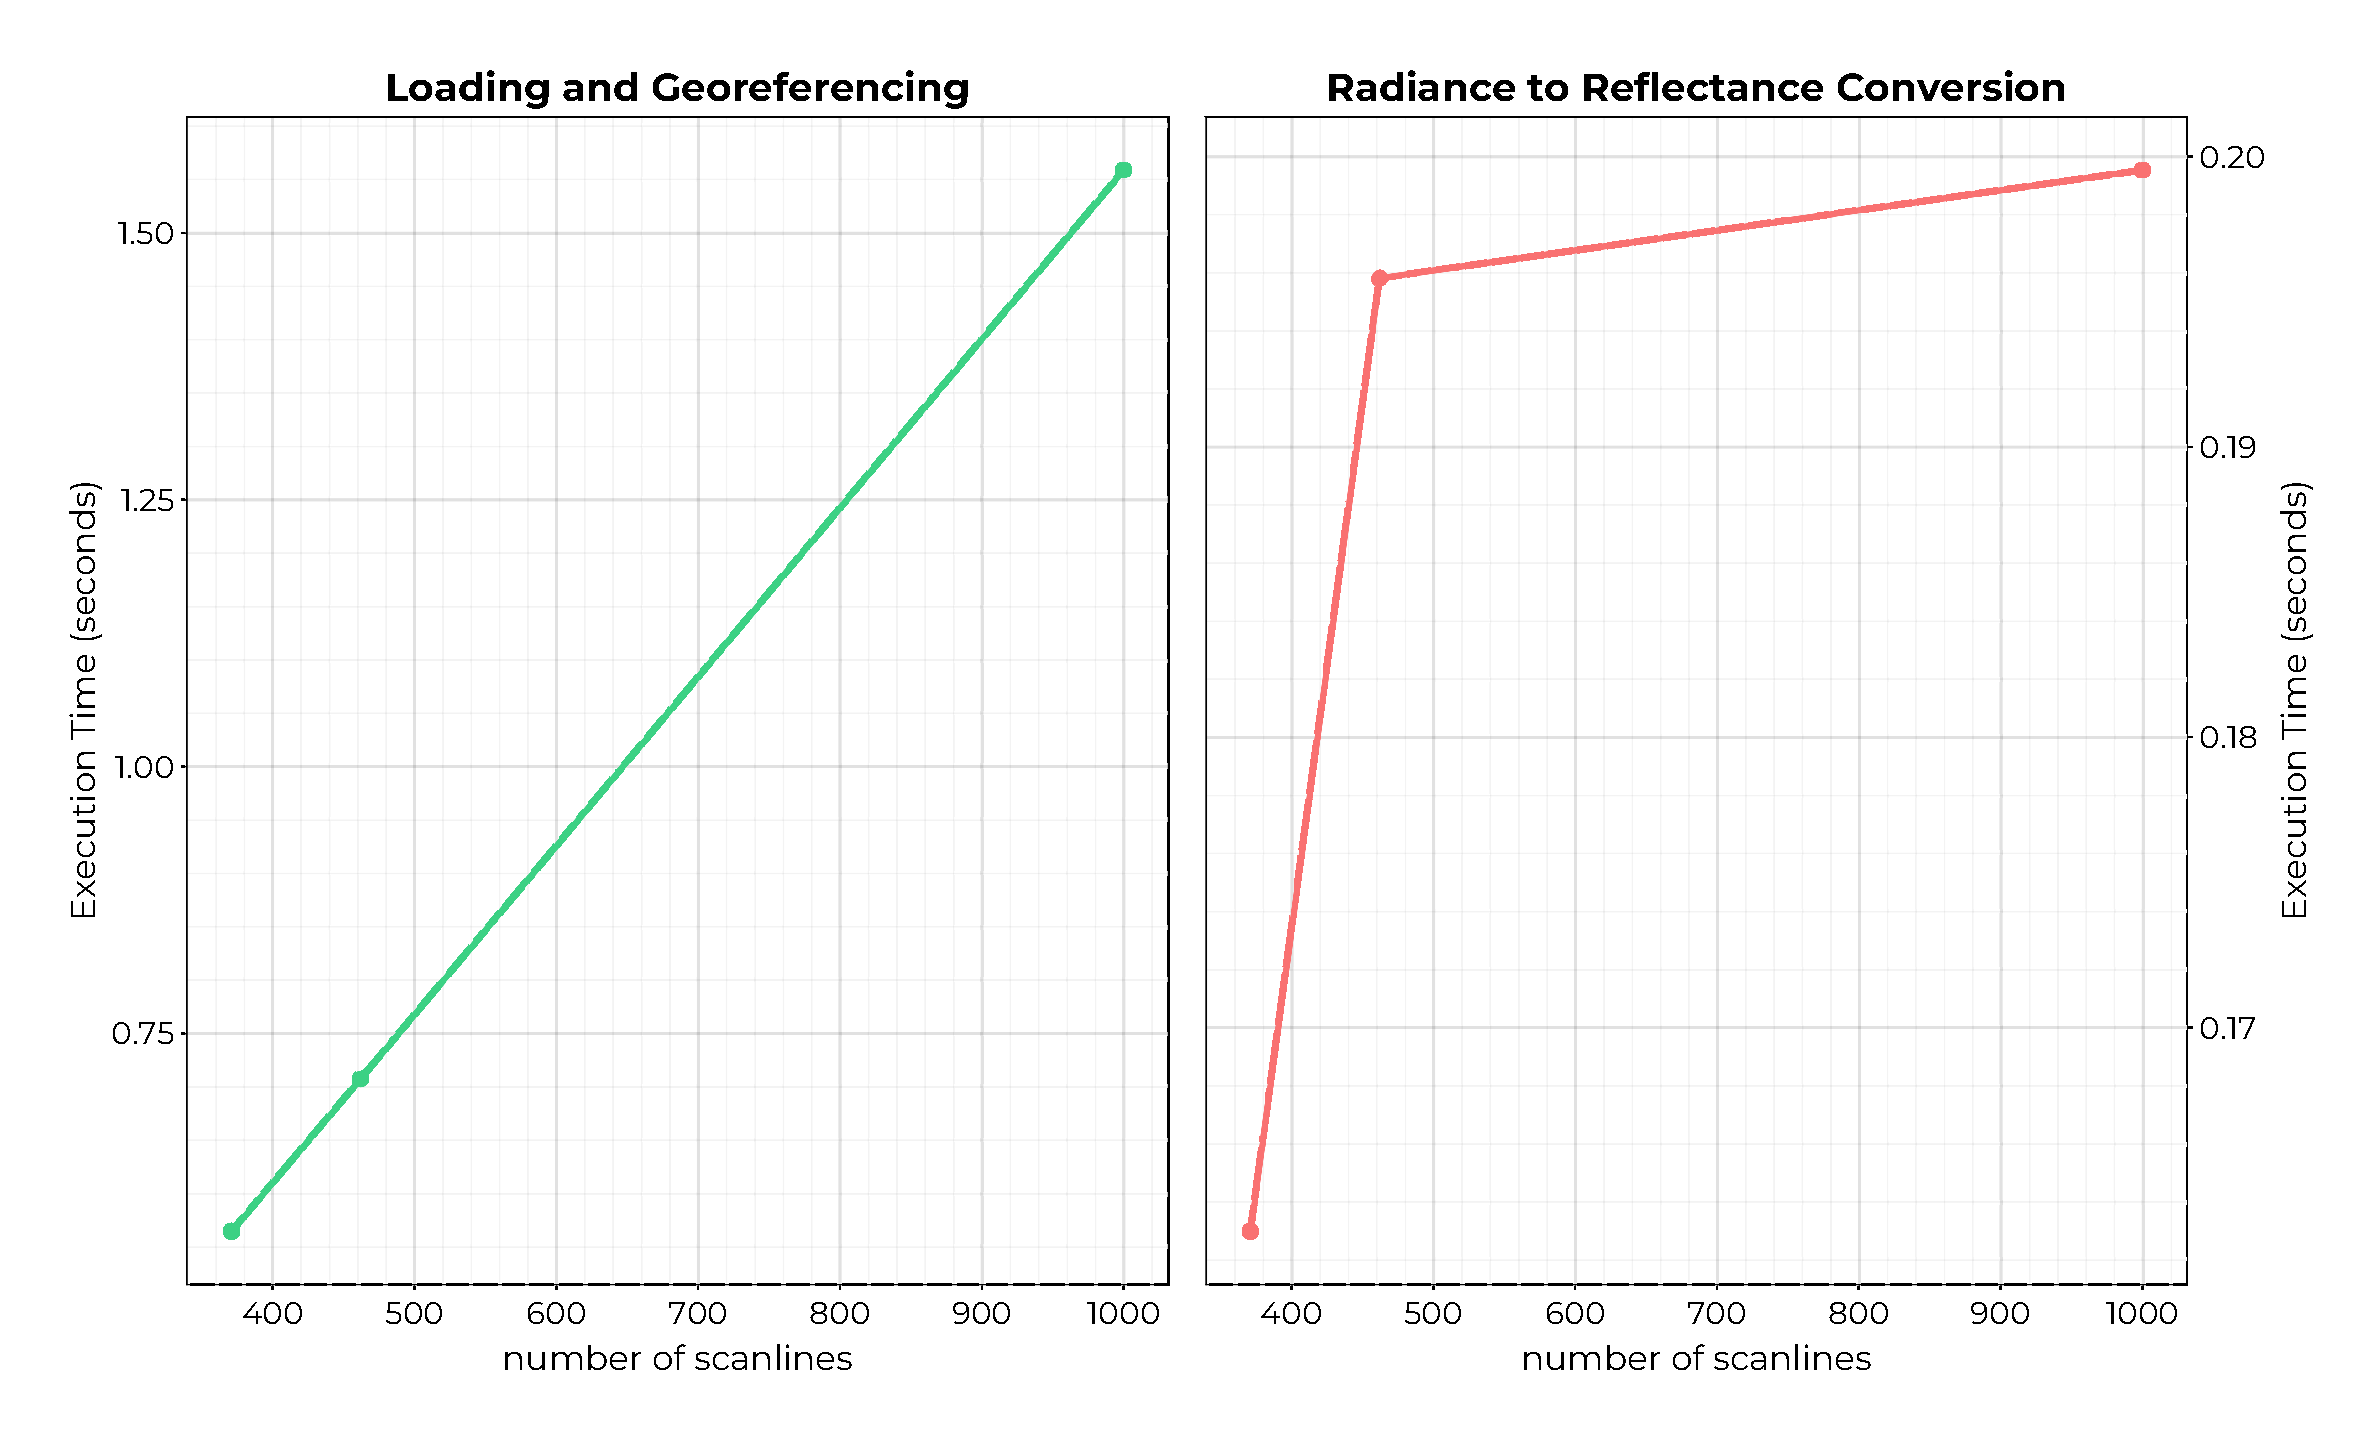
\includegraphics[width=10.5 cm]{./figures/reflectance-timing.eps}
  \caption{Description \label{fig-reflectance-timing}}
\end{figure}

NOTE: we need to update these timings by first copying the HSI to the local drive (off of the external hard drive). This will probably have some effect on the read/write speeds for the test.

\begin{table}[H]
\caption{Resampling times as a function of pixel resolution.\label{tab1}}
\newcolumntype{C}{>{\centering\arraybackslash}X}
\begin{tabularx}{\textwidth}{CC}
\toprule
\textbf{Resolution (m)}	& \textbf{Execution time (s)}\\
\midrule
0.5		&   1.434	\\
0.4     &   1.545	\\
0.3     &   1.673   \\
0.2     &   1.802   \\
0.1     &   4.026   \\
0.05    &   10.537  \\ 
\bottomrule
\end{tabularx}
\end{table}


\begin{table}[H]
  \caption{Loading and Reflectance Conversion Times.\label{tab1}}
  \newcolumntype{C}{>{\centering\arraybackslash}X}
  \begin{tabularx}{\textwidth}{CC}
    \toprule
    \textbf{Number of scan lines}	& \textbf{Execution time (s)}\\
    \midrule
    371		&   2.060	\\
    725     &   4.227	\\
    1000    &   5.901   \\
    \bottomrule
  \end{tabularx}
\end{table}




\textbf{NOTE} Stuff to do in this section:
\begin{itemize}
    \item  Create table with processing timings for each step on a typical HSI
    \item Create second table comparing time for full processing including resampling to a variety of scales (e.g. 5 cm, 10 cm, 25 cm) We will want a version of the processing function that does not include the uncertainties and the spectral indices
    \item create pipeline visualization showing size of each of the data products and their step in the pipeline (ending with a dataproduct like the NDVI)
    \item Create a figure showing the georeferenced image on top of the satellite background 
    \item Create another figure of the entire map with a spectral index applied to one of the dye-release datasets (to demonstrate use for real-time application like oil-spill)
    \item create a figure of a sample HSI datacube in 3-d like from the previous paper with the rgb image on the top. 
\end{itemize}



%%%%%%%%%%%%%%%%%%%%%%%%%%%%%%%%%%%%%%%%%%
\section{Discussion}

- Incorporation of drone into autonomous robotic team
- Long range wireless network (ubiquiti) for data downlink
- Incorporation of edge-ML for direct determination of chemical concentration
- Utility for navigation, waste removal, etc...

Discuss drawbacks (striping in images) 

Authors should discuss the results and how they can be interpreted from the perspective of previous studies and of the working hypotheses. The findings and their implications should be discussed in the broadest context possible. Future research directions may also be highlighted.

\begin{figure}[H]
    \includegraphics[width=10.5 cm]{./figures/mNDWI_example.png}
\caption{Sample data product created on-board the aerial vehicle. The modified normalized difference water index is computed for each HSI and combined into a map. The plume of Rhodamine dye can clearly be seen in the water.\label{fig-map}}
\end{figure}

%%%%%%%%%%%%%%%%%%%%%%%%%%%%%%%%%%%%%%%%%%
\section{Conclusions}

This section is not mandatory, but can be added to the manuscript if the discussion is unusually long or complex.

%%%%%%%%%%%%%%%%%%%%%%%%%%%%%%%%%%%%%%%%%%
\section{Patents}

This section is not mandatory, but may be added if there are patents resulting from the work reported in this manuscript.

%%%%%%%%%%%%%%%%%%%%%%%%%%%%%%%%%%%%%%%%%%
\vspace{6pt} 

%%%%%%%%%%%%%%%%%%%%%%%%%%%%%%%%%%%%%%%%%%
%% optional
%\supplementary{The following supporting information can be downloaded at:  \linksupplementary{s1}, Figure S1: title; Table S1: title; Video S1: title.}

% Only for the journal Methods and Protocols:
% If you wish to submit a video article, please do so with any other supplementary material.
% \supplementary{The following supporting information can be downloaded at: \linksupplementary{s1}, Figure S1: title; Table S1: title; Video S1: title. A supporting video article is available at doi: link.}

%%%%%%%%%%%%%%%%%%%%%%%%%%%%%%%%%%%%%%%%%%
\authorcontributions{For research articles with several authors, a short paragraph specifying their individual contributions must be provided. The following statements should be used ``Conceptualization, X.X. and Y.Y.; methodology, X.X.; software, X.X.; validation, X.X., Y.Y. and Z.Z.; formal analysis, X.X.; investigation, X.X.; resources, X.X.; data curation, X.X.; writing---original draft preparation, X.X.; writing---review and editing, X.X.; visualization, X.X.; supervision, X.X.; project administration, X.X.; funding acquisition, Y.Y. All authors have read and agreed to the published version of the manuscript.'', please turn to the  \href{http://img.mdpi.org/data/contributor-role-instruction.pdf}{CRediT taxonomy} for the term explanation. Authorship must be limited to those who have contributed substantially to the work~reported.}

\funding{Please add: ``This research received no external funding'' or ``This research was funded by NAME OF FUNDER grant number XXX.'' and  and ``The APC was funded by XXX''. Check carefully that the details given are accurate and use the standard spelling of funding agency names at \url{https://search.crossref.org/funding}, any errors may affect your future funding.}

\institutionalreview{In this section, you should add the Institutional Review Board Statement and approval number, if relevant to your study. You might choose to exclude this statement if the study did not require ethical approval. Please note that the Editorial Office might ask you for further information. Please add “The study was conducted in accordance with the Declaration of Helsinki, and approved by the Institutional Review Board (or Ethics Committee) of NAME OF INSTITUTE (protocol code XXX and date of approval).” for studies involving humans. OR “The animal study protocol was approved by the Institutional Review Board (or Ethics Committee) of NAME OF INSTITUTE (protocol code XXX and date of approval).” for studies involving animals. OR “Ethical review and approval were waived for this study due to REASON (please provide a detailed justification).” OR “Not applicable” for studies not involving humans or animals.}

\informedconsent{Any research article describing a study involving humans should contain this statement. Please add ``Informed consent was obtained from all subjects involved in the study.'' OR ``Patient consent was waived due to REASON (please provide a detailed justification).'' OR ``Not applicable'' for studies not involving humans. You might also choose to exclude this statement if the study did not involve humans.

Written informed consent for publication must be obtained from participating patients who can be identified (including by the patients themselves). Please state ``Written informed consent has been obtained from the patient(s) to publish this paper'' if applicable.}

\dataavailability{We encourage all authors of articles published in MDPI journals to share their research data. In this section, please provide details regarding where data supporting reported results can be found, including links to publicly archived datasets analyzed or generated during the study. Where no new data were created, or where data is unavailable due to privacy or ethical re-strictions, a statement is still required. Suggested Data Availability Statements are available in section “MDPI Research Data Policies” at \url{https://www.mdpi.com/ethics}.} 

\acknowledgments{In this section you can acknowledge any support given which is not covered by the author contribution or funding sections. This may include administrative and technical support, or donations in kind (e.g., materials used for experiments).}

\conflictsofinterest{Declare conflicts of interest or state ``The authors declare no conflict of interest.'' Authors must identify and declare any personal circumstances or interest that may be perceived as inappropriately influencing the representation or interpretation of reported research results. Any role of the funders in the design of the study; in the collection, analyses or interpretation of data; in the writing of the manuscript; or in the decision to publish the results must be declared in this section. If there is no role, please state ``The funders had no role in the design of the study; in the collection, analyses, or interpretation of data; in the writing of the manuscript; or in the decision to publish the~results''.} 

%%%%%%%%%%%%%%%%%%%%%%%%%%%%%%%%%%%%%%%%%%
%% Optional
\sampleavailability{Samples of the compounds ... are available from the authors.}

%% Only for journal Encyclopedia
%\entrylink{The Link to this entry published on the encyclopedia platform.}

\abbreviations{Abbreviations}{
The following abbreviations are used in this manuscript:\\

\noindent 
\begin{tabular}{@{}ll}
MDPI & Multidisciplinary Digital Publishing Institute\\
DOAJ & Directory of open access journals\\
TLA & Three letter acronym\\
LD & Linear dichroism
\end{tabular}
}

%%%%%%%%%%%%%%%%%%%%%%%%%%%%%%%%%%%%%%%%%%
%% Optional
\appendixtitles{no} % Leave argument "no" if all appendix headings stay EMPTY (then no dot is printed after "Appendix A"). If the appendix sections contain a heading then change the argument to "yes".
\appendixstart
\appendix
\section[\appendixname~\thesection]{}
\subsection[\appendixname~\thesubsection]{}
The appendix is an optional section that can contain details and data supplemental to the main text---for example, explanations of experimental details that would disrupt the flow of the main text but nonetheless remain crucial to understanding and reproducing the research shown; figures of replicates for experiments of which representative data are shown in the main text can be added here if brief, or as Supplementary Data. Mathematical proofs of results not central to the paper can be added as an appendix.

\begin{table}[H] 
\caption{This is a table caption.\label{tab5}}
\newcolumntype{C}{>{\centering\arraybackslash}X}
\begin{tabularx}{\textwidth}{CCC}
\toprule
\textbf{Title 1}	& \textbf{Title 2}	& \textbf{Title 3}\\
\midrule
Entry 1		& Data			& Data\\
Entry 2		& Data			& Data\\
\bottomrule
\end{tabularx}
\end{table}

\section[\appendixname~\thesection]{}
All appendix sections must be cited in the main text. In the appendices, Figures, Tables, etc. should be labeled, starting with ``A''---e.g., Figure A1, Figure A2, etc.

%%%%%%%%%%%%%%%%%%%%%%%%%%%%%%%%%%%%%%%%%%
\begin{adjustwidth}{-\extralength}{0cm}
%\printendnotes[custom] % Un-comment to print a list of endnotes

\reftitle{References}

% Please provide either the correct journal abbreviation (e.g. according to the “List of Title Word Abbreviations” http://www.issn.org/services/online-services/access-to-the-ltwa/) or the full name of the journal.
% Citations and References in Supplementary files are permitted provided that they also appear in the reference list here. 

%=====================================
% References, variant A: external bibliography
%=====================================
%\bibliography{your_external_BibTeX_file}

%=====================================
% References, variant B: internal bibliography
%=====================================
\begin{thebibliography}{999}
% Reference 1
\bibitem[Author1(year)]{ref-journal}
Author~1, T. The title of the cited article. {\em Journal Abbreviation} {\bf 2008}, {\em 10}, 142--149.
% Reference 2
\bibitem[Author2(year)]{ref-book1}
Author~2, L. The title of the cited contribution. In {\em The Book Title}; Editor 1, F., Editor 2, A., Eds.; Publishing House: City, Country, 2007; pp. 32--58.
% Reference 3
\bibitem[Author3(year)]{ref-book2}
Author 1, A.; Author 2, B. \textit{Book Title}, 3rd ed.; Publisher: Publisher Location, Country, 2008; pp. 154--196.
% Reference 4
\bibitem[Author4(year)]{ref-unpublish}
Author 1, A.B.; Author 2, C. Title of Unpublished Work. \textit{Abbreviated Journal Name} year, \textit{phrase indicating stage of publication (submitted; accepted; in press)}.
% Reference 5
\bibitem[Author5(year)]{ref-communication}
Author 1, A.B. (University, City, State, Country); Author 2, C. (Institute, City, State, Country). Personal communication, 2012.
% Reference 6
\bibitem[Author6(year)]{ref-proceeding}
Author 1, A.B.; Author 2, C.D.; Author 3, E.F. Title of presentation. In Proceedings of the Name of the Conference, Location of Conference, Country, Date of Conference (Day Month Year); Abstract Number (optional), Pagination (optional).
% Reference 7
\bibitem[Author7(year)]{ref-thesis}
Author 1, A.B. Title of Thesis. Level of Thesis, Degree-Granting University, Location of University, Date of Completion.
% Reference 8
\bibitem[Author8(year)]{ref-url}
Title of Site. Available online: URL (accessed on Day Month Year).
\end{thebibliography}

% If authors have biography, please use the format below
%\section*{Short Biography of Authors}
%\bio
%{\raisebox{-0.35cm}{\includegraphics[width=3.5cm,height=5.3cm,clip,keepaspectratio]{Definitions/author1.pdf}}}
%{\textbf{Firstname Lastname} Biography of first author}
%
%\bio
%{\raisebox{-0.35cm}{\includegraphics[width=3.5cm,height=5.3cm,clip,keepaspectratio]{Definitions/author2.jpg}}}
%{\textbf{Firstname Lastname} Biography of second author}

% For the MDPI journals use author-date citation, please follow the formatting guidelines on http://www.mdpi.com/authors/references
% To cite two works by the same author: \citeauthor{ref-journal-1a} (\citeyear{ref-journal-1a}, \citeyear{ref-journal-1b}). This produces: Whittaker (1967, 1975)
% To cite two works by the same author with specific pages: \citeauthor{ref-journal-3a} (\citeyear{ref-journal-3a}, p. 328; \citeyear{ref-journal-3b}, p.475). This produces: Wong (1999, p. 328; 2000, p. 475)

%%%%%%%%%%%%%%%%%%%%%%%%%%%%%%%%%%%%%%%%%%
%% for journal Sci
%\reviewreports{\\
%Reviewer 1 comments and authors’ response\\
%Reviewer 2 comments and authors’ response\\
%Reviewer 3 comments and authors’ response
%}
%%%%%%%%%%%%%%%%%%%%%%%%%%%%%%%%%%%%%%%%%%
\PublishersNote{}
\end{adjustwidth}
\end{document}

